 
\documentclass[12pt]{article}
%authors Andrew Schneider, David Dobor
\usepackage[margin=1in]{geometry} 
\usepackage{amsmath,amsthm,amssymb}
 \usepackage{graphicx}
 \usepackage{multirow}
\usepackage[scaled]{helvet}
\usepackage{hyperref}
\usepackage[usenames,dvipsnames,svgnames,table]{xcolor}
\usepackage[T1]{fontenc}
\usepackage{palatino}
\usepackage{enumerate}
%\renewcommand*\familydefault{\sfdefault} %% Only if the base font of the document is to be sans serif

\newcommand{\N}{\mathbb{N}}
\newcommand{\Z}{\mathbb{Z}}


\newcommand{\blditA}{\textbf{\textit{A}}}
\newcommand{\blditB}{\textbf{\textit{B}}}
\newcommand{\blditC}{\textbf{\textit{C}}}
\newcommand{\blditP}{\textbf{\textit{P}}}
\newcommand{\blditQ}{\textbf{\textit{Q}}}
\newcommand{\bldI}{\textbf{I}}
\newcommand{\blditX}{\textbf{\textit{X}}}
\newcommand{\blditY}{\textbf{\textit{Y}}}
\newcommand{\blditZ}{\textbf{\textit{Z}}}
 
\newenvironment{theorem}[2][Theorem]{\begin{trivlist}
\item[\hskip \labelsep {\bfseries #1}\hskip \labelsep {\bfseries #2.}]}{\end{trivlist}}
\newenvironment{lemma}[2][Lemma]{\begin{trivlist}
\item[\hskip \labelsep {\bfseries #1}\hskip \labelsep {\bfseries #2.}]}{\end{trivlist}}
\newenvironment{exercise}[2][Exercise]{\begin{trivlist}
\item[\hskip \labelsep {\bfseries #1}\hskip \labelsep {\bfseries #2.}]}{\end{trivlist}}
\newenvironment{problem}[2][Problem]{\begin{trivlist}
\item[\hskip \labelsep {\bfseries #1}\hskip \labelsep {\bfseries #2.}]}{\end{trivlist}}
\newenvironment{question}[2][Question]{\begin{trivlist}
\item[\hskip \labelsep {\bfseries #1}\hskip \labelsep {\bfseries #2.}]}{\end{trivlist}}
\newenvironment{answer}[2][Answer]{\begin{trivlist}
\item[\hskip \labelsep {\bfseries #1}\hskip \labelsep {\bfseries #2.}]}{\end{trivlist}}

\begin{document}
 \renewcommand{\arraystretch}{1.3}

 
\title{Stat 8003, Homework 6}%replace X with the appropriate number
\author{Group G: \ \ \texttt{sample( c( "David" , "Andrew",  "Salam" ))}
\\ %replace with your name
} %if necessary, replace with your course title
 
\maketitle
 
 %%%%%%%% Question 1 %%%%%%%%%
 \begin{question}{6.1}  A coin is thrown independently 10 times to test the hypothesis that the probability of heads is
1/2 versus the alternative that the probability is not 1/2. The test rejects if either 0 or 10 heads
are observed.

\begin{enumerate}[(a)]
\item What is the significance level of the test?
\item If in fact the probability of heads is .1, what is the power of the test?
\end{enumerate}

\end{question} 


  \textbf{\color{TealBlue}\emph{Answer:} } 
 \begin{enumerate}[(a)]  
\item Let $X$ be the number of heads showing up in 10 tosses of the coin, i.e. $X \sim Binomial(10, p)$ where $p$ is the probability of landing heads. The hypotheses are
$$ 
H_0: \ p = \frac{1}{2}, \; \; \; \; vs  \; \; \; \; H_a: \ p  \neq \frac{1}{2}.
$$
By definition,
\begin{align*}
\alpha &= P (X = 0 \mid H_0) + P (X = 10 \mid H_0) \\
&= {10 \choose 0} \left(\frac{1}{2}\right)^0 \left(\frac{1}{2}\right)^{10} +  {10 \choose 10} \left(\frac{1}{2}\right)^{10} \left(\frac{1}{2}\right)^{0}\\
&= \frac{2}{2^{10}}  = \frac{1}{512}\\
&= 0.002
\end{align*}

\item If $p = 0.1$, then the probability of rejecting the null hypothesis is
\begin{align*}
1 - \beta &= {10 \choose 0} (0.1)^0 (0.9)^{10} +  {10 \choose 10} (0.1)^{10} (0.9)^{0}\\
&= 0.3486784
\end{align*}
Thus the significance level of this test is 0.002 and its power is 0.3487.
\end{enumerate}
\bigskip
\bigskip
 %%%%%%%% Question 2 %%%%%%%%%
 \begin{question}{6.2}  Let $X_1, · · · ,X_n$ be a random sample from an exponential distribution with the density function
$$
f(x \mid \theta) = \theta \mathrm{e}^{-\theta x}.
$$
We want to test the hypothesis
$$
H_0: \ \theta = 1, \; \; \; \; vs  \; \; \; \; H_a: \ \theta \neq 1.
$$
Set the desired level of significance as $\alpha = 5\%$.

\begin{enumerate}[(a)]
\item Derive a generalized likelihood ratio test and show that the rejection region is of the form $\mathcal{R} = \{\bar X \mathrm{e}^{-\bar X} \leq c\}$;
\item Suppose n = 10. Show that the rejection region in (a) is of the form $\mathcal{R} = \{\bar X \leq x_0 \} \cup \{\bar X \geq x_1 \}$, where $x_0$ and $x_1$ are determined by $c$;
\item When $\theta = 1$, it is known that $\sum_i X_i$ follows $Gamma(n, \frac{1}{\theta})$. How could this knowledge be
used to choose $c$?
\end{enumerate}

\end{question} 

  \textbf{\color{TealBlue}\emph{Answer:} } 

\begin{enumerate}[(a)]

%%answer to 2 (a)
\item Since the \texttt{MLE} of the parameter $\theta$ for the exponential distribuiton is given by:
$$
\hat \theta = 1 / \bar X,
$$
We have that the \texttt{GLRT} is given by:
\begin{align*}
\Lambda &= \frac{max_{\theta \in \Theta_0 \cup \Theta_1} L(\theta; x) } {max_{\theta \in \Theta_0} L(\theta; x)  }
= \frac{max_{\theta \in \Theta_0 \cup \Theta_1} \theta^n \mathrm{e}^{-\theta \sum_i x_i} } {max_{\theta \in \Theta_0} \theta^n \mathrm{e}^{-\theta \sum_i x_i} }\\
&= \frac{(1 / \bar X)^n \mathrm{e}^{- 1/ \bar X \sum_i x_i }} {\theta_0^n \mathrm{e}^{-\theta_0 \sum_i x_i}} \\
&= \frac{(1 / \bar X)^n \mathrm{e}^{(- 1/ \bar X) \ n \ (\sum_i x_i / n) }}{1^n \mathrm{e}^{-1 \ \sum_i x_i}} \\
&=  \frac{(1 / \bar X)^n \mathrm{e}^{-n} } {\mathrm{e}^{-n \ (\sum_i x_i) / n}} \\
&= (1 / \bar X)^n \mathrm{e}^{ -n } \mathrm{e}^{n \bar X} \\
\end{align*}
Our criterion for rejecting the Null Hypothesis is that this ratio be greater than some constant:
$$
\Lambda \geq k^*
$$
We can simplify the above expression for $\Lambda$ further by taking the $n$-th root of both sides of this expression:
\begin{align*}
\Lambda^{\frac{1}{n}}  &=  \left( (1 / \bar X)^n \mathrm{e}^{ -n } \mathrm{e}^{n \bar X} \right)^{\frac{1}{n}}\\
&\geq  (k^*)^{\frac{1}{n}}
\end{align*}
$\Rightarrow$
\begin{align*}
 (1 / \bar X) \mathrm{e}^{ -1 } \mathrm{e}^{\bar X} & \geq (k^*)^{\frac{1}{n}} \\
\end{align*}
$\Rightarrow$
\begin{align*}
 \frac{1} {(1 / \bar X) \mathrm{e}^{\bar X}} =\bar X \mathrm{e}^{-\bar X}  & \leq \frac{1} {(k^*)^{\frac{1}{n}} \mathrm{e}} = c \\
\end{align*}
Thus we have shown that the rejection region $\mathcal{R}$ is given by:
$$
\boxed{\bar X \mathrm{e}^{-\bar X} \leq \ \text{some constant} \; c }
$$
\bigskip

%%answer to 2 (b)
\item
Some people like to claim that a picture is worth a few words\footnote{One author of this homework has heard of pictures being worth thousands of words, but he's skeptical of this claim.}. Here's what the rejection region from part (a) might look like:

\begin{center}
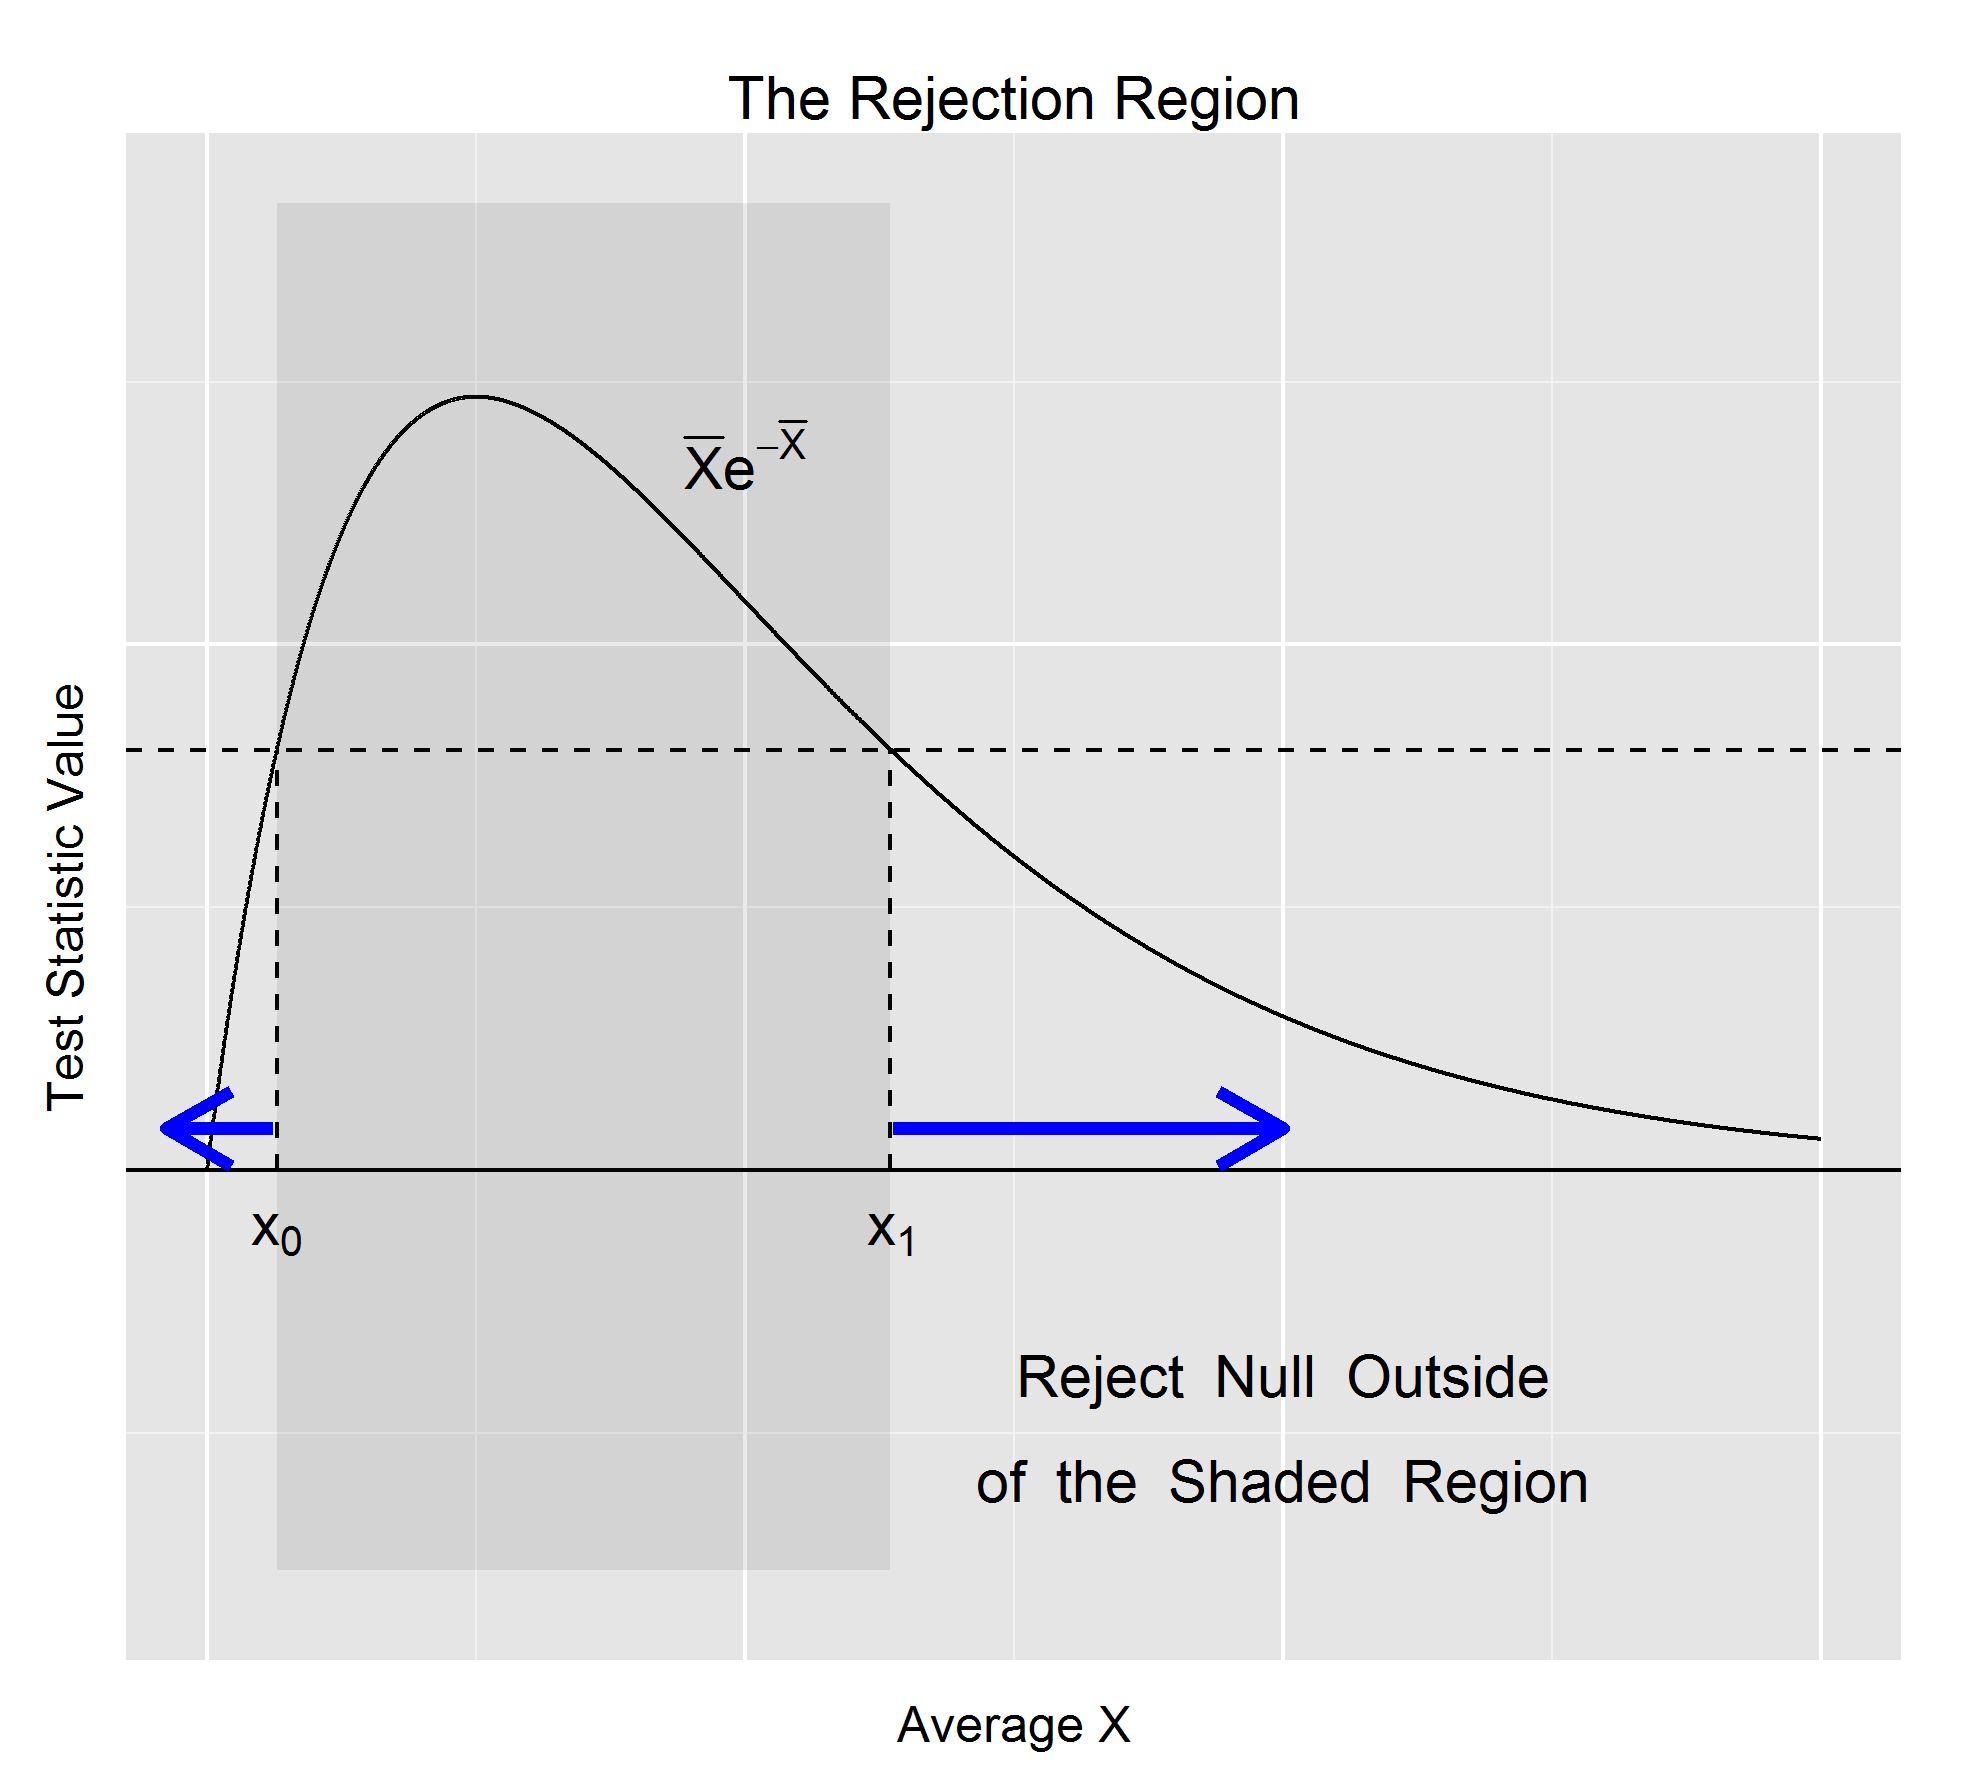
\includegraphics[width=10cm, height=10cm]{rejection_region_plot}
\end{center} 

The dashed horizontal line in this picture corresponds to the constant $c$ from part (a). The test statistic has to be below this constant, that is $\bar X$ has to fall outside the shaded region, for us to reject $H_0$. This picture shows that $x_0$ and $x_1$ are determined by the constant $c$: at these points our test statistic $\bar X \mathrm{e}^{-\bar X}$ intersects the horizontal line at level $c$.
\bigskip
%%answer to 2 (c)
\item
To simplify the notation, let $Y = \sum_i^{10} X_i$. We know that under the null hypothesis $Y$ follows the $Gamma(10, 1)$ distribution. We rewrite the expression we got in part (a) as follows:
\begin{align*}
\bar X \mathrm{e}^{-\bar X} \leq c \; \; \; &\Rightarrow \; \; \; \frac{Y}{10} (\mathrm{e}^{-Y})^{\frac{1}{10}} \leq c\\
\\
&\Rightarrow \; \; \; Y^{10} \mathrm{e}^{-Y} \leq (10 c)^{10} \\
\end{align*}

Thus we are looking for a constant $c$ such that 
$$
P \left( Y^{10} \mathrm{e}^{-Y} \leq (10 c)^{10} \right)  = \alpha = 0.05.
$$
Or, taking the logarithms of both sides of the inequality,
$$
P \left(  10 \log Y - Y \leq \log \left( (10 c)^{10} \right) \right) = 0.05.
$$
Again, for simplicity of notation, denote $\log( (10 c)^{10}) $ by $k$. Thus, for $Y \sim Gamma(10,1)$, we are looking for such constant $k$ that satisfies the following inequality:
$$
\boxed{P \left( \  10 \log Y - Y \leq k \  \right) = 0.05}
$$

We can plot $ 10 \log Y - Y $ and find the constant $k$ that makes the area under the curve, and below this constant, equal to $\alpha = 0.05$. (We can then easily recover $c$ from $k$, if need be).

\begin{center}
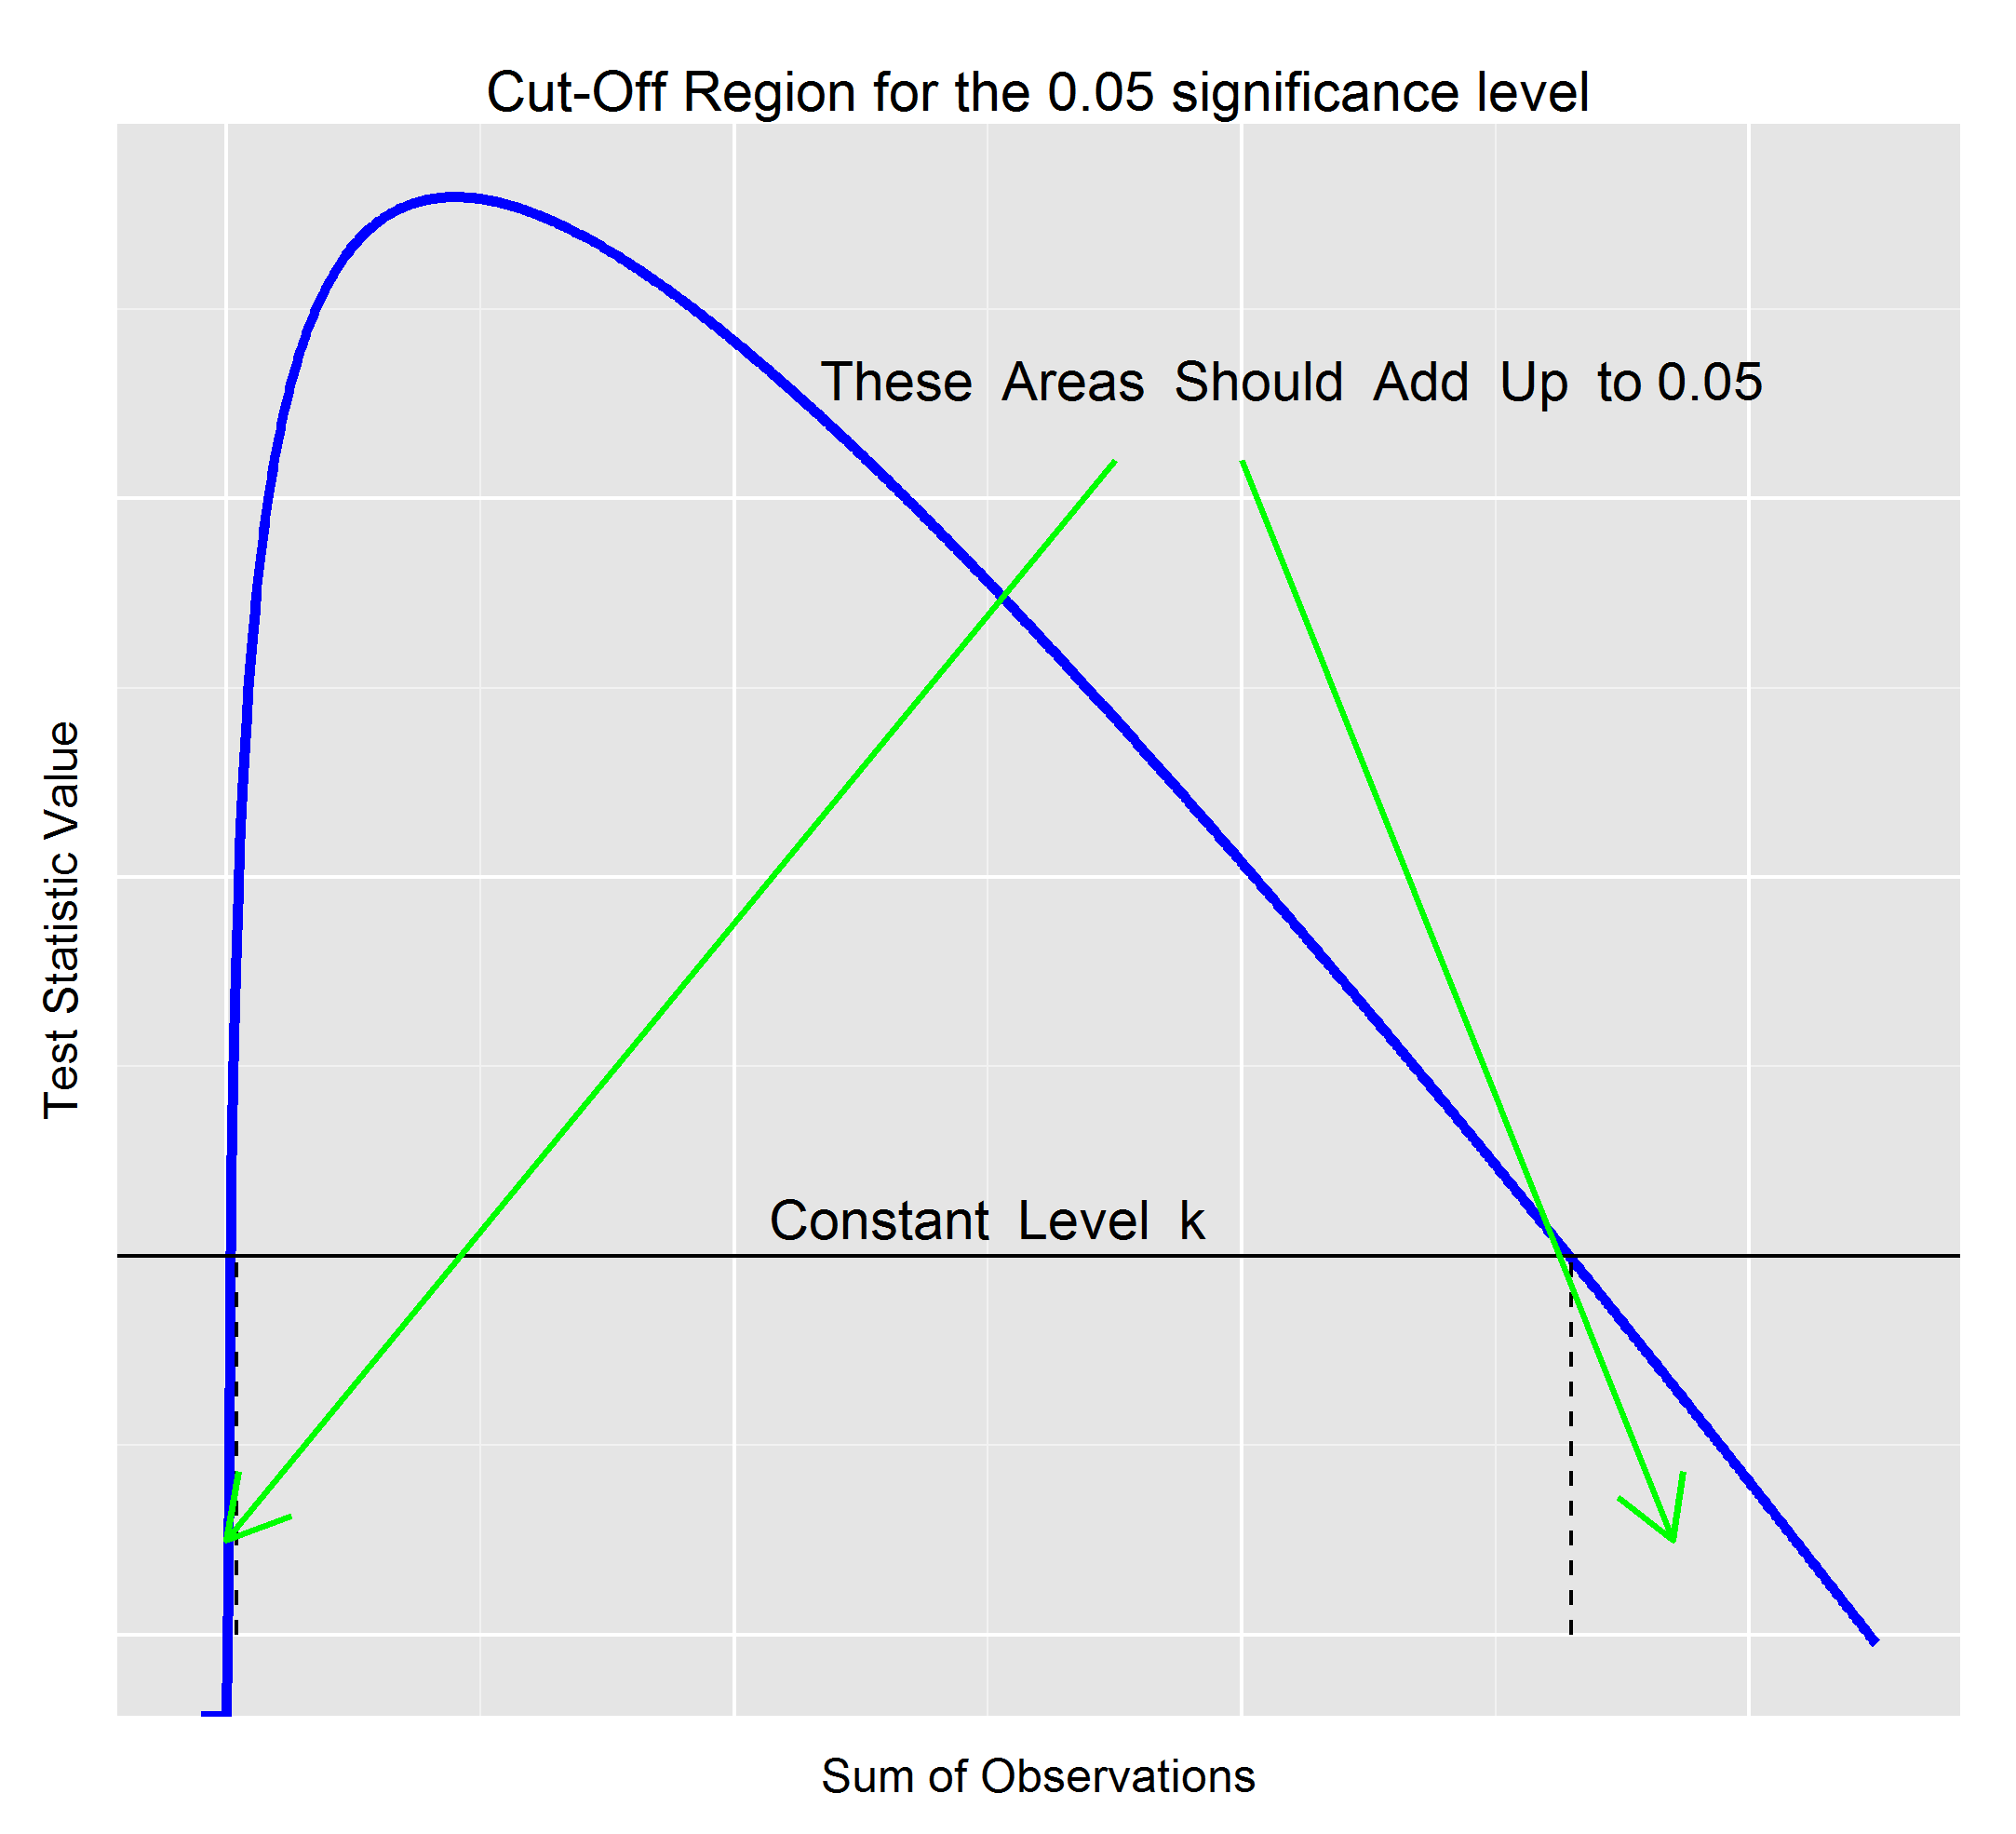
\includegraphics[width=10cm, height=10cm]{alpha_cut_off}
\end{center} 
\end{enumerate}


\bigskip
\bigskip
 %%%%%%%% Question 3 %%%%%%%%%
 \begin{question}{6.3}Suppose, to be specific, that in Problem 2, the observed data are the following:
\begin{verbatim}
1.07 0.88 0.66 0.55 1.15 0.65 3.45 3.55 3.51 0.48
\end{verbatim}

\begin{enumerate}[(a)]
\item Based on the result in Problem 2, will you reject $H_0$? What's your $p$-value?
\item If we start from generalized likelihood ratio test, and use the asymptotic distribution of $2 \log \Lambda$, will you reject $H_0$? What's you $p$-value?
\end{enumerate}

\end{question} 


  \textbf{\color{TealBlue}\emph{Answer:} } 
 

\end{document}

